% Maybe need something involving sets still
% Probably can't have too much Turing machine stuff if it's optional. 

\documentclass[12pt]{article}
\usepackage[utf8]{inputenc}
\usepackage[margin=0.8in]{geometry}
\usepackage{ragged2e}
\usepackage{amsmath,amssymb}
\usepackage{minted}
\usepackage{listings}
\usepackage{tikz}
\usetikzlibrary{chains,fit,shapes}

\title{CSCI 3383 \\Midterm Exam}
\date{}

\begin{document}
\maketitle
\textbf{\emph{Full, printed} name: }
\vspace{1cm}
% finding loop invariant
% big O and the gang
\textbf{Instructions}: 
\begin{itemize}
    \item Read the instructions
    \item Stuck? I will allow everyone \textbf{one} hint during the exam. Raise your hand and I will try to get you moving in the right direction.  
    \item You are allowed scratch paper and a calculator. 
    \item Have a wonderful holiday break!
\end{itemize} 

\newpage
\begin{enumerate}
    \item[(1)] If algorithm A runs in time $O(n^2)$, and algorithm B runs in time $O(n^3)$, then algorithm A is always the faster option.
        \begin{itemize}
            \item[(a)] True
            \item[(b)] False
        \end{itemize}
    \item[(2)] Suppose $f(k)$ is an algorithm which takes a single integer input $k$ and runs in time $O(n)$, where $n$ is the number of digits in $k$. Suppose you timed and ran $f$ on all possible $k$ between $1$ and $1000$, and then plotted the runtimes with respect to $k$. You would expect to see a 
    \begin{itemize}
        \item[(a)] Linear curve
        \item[(b)] Logarithmic curve 
        \item[(c)] Parabolic curve
        \item[(d)] Exponential curve
    \end{itemize}
    \item[(3)] No sorting algorithm can ever be faster than $O(n\log(n))$ in the worst-case.
    \begin{itemize}
        \item[(a)] True
        \item[(b)] False
    \end{itemize}
    \item[(4)] The claim that $\underset{n\to\infty}{\lim}\frac{f(n)}{g(n)} = c$ for some nonnegative $c$ is \underline{\hspace{1.3cm}} the claim that $f(n) = O(g(n))$.
    \begin{itemize}
        \item[(a)] stronger than
        \item[(b)] weaker than
        \item[(c)] equivalent to
    \end{itemize}
    \item[(5)] Identifying loop invariants is useful for proving the correctness of what kinds of code? (Select all that apply)
    \begin{itemize}
            \item[(a)] For loops
            \item[(b)] While loops
            \item[(c)] Recursion  
    \end{itemize}
    \item[(5)] In what situation would it be a good idea to make a list into a heap? In what situation would it be a bad idea? 
    \newpage 
    \item[(6)] State whether the following claims are true or false, and justify your answers:
    \begin{itemize}
        \item[(a)] $3n^4+5n^2+\sqrt{n} = O(n^4)$ \vspace{4cm}
        \item[(b)] $3n^4+5n^2+\sqrt{n} = \Theta(n^4)$ \vspace{4cm}
        \item[(c)] $3n^4+5n^2+\sqrt{n} = \omega(n^4)$ \vspace{4cm}
        \item[(c)] $\log(n) = o(n)$ \vspace{3cm}
        \item[(d)] $n\log(n) = O(n^1.001)$ \vspace{3cm}
        \item[(e)] $3^n = O(2^n)$ \vspace{3cm}
    \end{itemize}
    \newpage
    \item[(7)] Consider the following function:
        \begin{lstlisting}
            def time_waster(array A, array B):
                some_num = 0
                for i in range(0,length(B)):
                    for j in range(0,length(A)):
                        sum_num += max(A)
                return some_num
        \end{lstlisting}
        Let $n = length(A)$, and $m = length(B)$. Express the following answers in terms of these variables.
        \begin{itemize}
            \item[(a)] What is the runtime of this function with respect to $A$ only? \vspace{3cm} % n^2 
            \item[(b)] What is the runtime of this function with respect to $B$ only? \vspace{3cm} % m
            \item[(c)] What is the runtime of this function with respect to both $A$ and $B$? \vspace{3cm}
        \end{itemize}
    \item[(8)] State a recurrence relation for the following code:
        \begin{lstlisting}
        def fun(array A):
            n = length(A)
            for i in range(0,n):
                A[i] = A[i] + 2
            return fun(A[1:n])
        \end{lstlisting}
    \newpage
    \item[(9)] Solve the following recurrence relations by any means:
    \begin{itemize}
        \item[(a)] $T(n) = 2T(\frac{n}{3}) + 1$ \vspace{4cm}
        \item[(b)] $T(n) = 5T(\frac{n}{4}) + n$ \vspace{4cm}
        \item[(c)] $T(n) = 7T(\frac{n}{7}) + n$ \vspace{4cm}
        \item[(d)] $T(n) = 9T(\frac{n}{3}) + n^2$ \vspace{4cm}
        \item[(e)] (Extra Credit) $T(n) = T(n-1) + n^3$ \vspace{4cm}
    \end{itemize}
    \newpage
    \item[(10)] State a sorting algorithm which fits the given constraints:
    \begin{itemize}
        \item[(a)] Must be stable, and must sort in place. \vspace{2cm}
        \item[(b)] Must sort in place and be fast. \vspace{2cm}
        \item[(c)] Must be as fast as possible. Possible elements are known, and all elements are equally likely. \vspace{2cm}
        \item[(d)] Must be fast, and stable. \vspace{2cm}
        \item[(e)] Must be fast, and stable. Numbers are guaranteed to be a small number of digits. \vspace{2cm}
    \end{itemize}
    \newpage
    \item[(11)] Consider the array $A$ given here:
    \begin{center}
        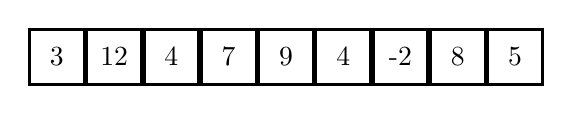
\begin{tikzpicture}
        \tikzstyle{every path}=[very thick]
        \edef\sizetape{0.7cm}
        \tikzstyle{tmtape}=[draw,minimum size=\sizetape]
        \tikzstyle{tmhead}=[arrow box,draw,minimum size=.5cm,arrow box
        arrows={north: .25cm}]
        \begin{scope}[start chain=1 going right,node distance=-0.15mm]
         \node [on chain=1,tmtape] {3};
         \node [on chain=1,tmtape] {12};
         \node [on chain=1,tmtape] {4};
         \node [on chain=1,tmtape] {7};
         \node [on chain=1,tmtape] {9};
         \node [on chain=1,tmtape] {4};
         \node [on chain=1,tmtape] {-2};
         \node [on chain=1,tmtape] {8};
         \node [on chain=1,tmtape] {5};
        \end{scope}
        \end{tikzpicture}
        \end{center}
    \begin{itemize}
        \item[(a)] Perform a partition of $A$ using the final element as the pivot. \vspace{10cm}
        \item[(b)] Draw the binary tree implicit to seeing $A$ as a heap, and then perform a max-heapify on it, indicating the sequence of swaps which would be performed and the final result, either as a new tree or as an array. \vspace{5cm}
    \end{itemize}
    \newpage
    \item[(11)] Suppose we wanted an algorithm $F(A,k)$ which, given an array $A$ and an integer $k$, would return the $k$ most frequently occuring elements of $A$. (The array elements need not be numbes. Let $n = length(A)$)
    \begin{itemize}
        \item[(a)] Briefly describe a brute-force solution to this problem, and state the big-O runtime. (No hash tables.) \vspace{7cm}
        \item[(b)] Describe a faster solution which makes use of the data structures we've discussed in class. You can simply reference the data structure operations by name without needing to write any code for them. State and justify your runtime in big-O notation. \vspace{7cm}
    \end{itemize}

    \newpage
    \item[(12)] 
    \begin{itemize}
        \item[(a)] Write pseudocode for the merge function which is used within the mergesort algorithm. \vspace{8cm}
        \item[(b)] Suppose we wanted an algorithm NoDupes(A) which, when given an array A, returns the same array but with all duplicate elements removed. Write pseudocode for a divide and conquer algorithm which solves this problem in time $O(n\log(n))$. Make sure to briefly justify why your algorithm operates in this time. (Hint: Can you modify the function from part a and make use of it?) \vspace{7cm}
    \end{itemize}

    % \item[(2)] Suppose we have three algorithms which solve the same problem. 
    % \begin{itemize}
    %     \item Algorithm $A$ solves the problem by dividing it into five subproblems, each of half the size of $A$, recursively solving each subproblem, then combining the solutions back together in linear time.
    %     \item Algorithm $B$ solves problems of size $n$ by recursively solving two subproblems of size $n-1$ and then combining the solutions in constant time. 
    %     \item Algorithm $C$ solves problems of size $n$ by dividing them into nine subproblems of size $\frac{n}{3}$, recursively solving each subproblem, and then combines the solutions in quadratic time. 
    % \end{itemize}
    % Which would you choose? Justify your answer by finding the runtimes of each.

\end{enumerate}
\end{document}